\documentclass{article}
%\usepackage[notref,notcite]{showkeys}

\usepackage{csvsimple-l3}
\usepackage{booktabs}
\usepackage{multirow}
\usepackage{graphicx}
\usepackage{biblatex}
\usepackage{listings}
\usepackage{siunitx}
\usepackage{pgfplots}
\usepackage{subcaption}
\usepackage{comment}
\usepackage{mathtools}
\usepackage{hyperref}

\pgfplotsset{compat=1.18}
\tikzset{ dots/.style = {mark=*, draw=black, mark size=.5pt} }
\usetikzlibrary{external}
\tikzexternalize
\addbibresource{bracket.bib}

\title{Seeding Statistics of Elimination Tournaments}
% Elimination Tournaments' Seeding Statistics
% Statistics of Seeding of Tournaments of Elimination   :-P
\author{Timothy Prescott\footnote{University of North Dakota}}
\date{\today}

\begin{document}

\maketitle

\tableofcontents

\begin{abstract}
We develop and provide Python code and a website to statistically analyze seedings in elimination tournaments.  We are able to apply this code to fifty-six thousand games to estimate the probability of an upset solely as a logistic function of the difference in seeding.  We are also able to examine how well or poorly a team performs compared to its seeding.  We conclude that the only team that is consistently underrated is \textbackslash your\_favorite\_team, while the only team that is consistently overrated is \textbackslash your\_hated\_rival.
\end{abstract}

\noindent
{\small\textbf{\textit{Keywords---}} logistic regression, statistical modeling, elimination tournament, Python}

\section{Introduction}
A notable occurrence during the 2024 NCAA Division I Men's Basketball Tournament (commonly known as March Madness) was that \#11 North Carolina State reached the Final Four, beating teams seeded 6, 14, 2, and 4.  Another notable occurrence was that the only upset in the first round of the women's tournament was by \#11 Middle Tennessee.  We will estimate that the probability of the first was 1.3\%, while the probability of the second was 2.4\%.

Bracket construction has been analyzed by \cite{Schwenk} and \cite{Seltzer}, while \cite{Wittry} examined upsets in the tournament.  Making accurate upset predictions is popular and profitable (see \cite{Chartier}), so that a driver of statistical research over the past few years has been to analyze teams' performance throughout the season in order to predict more accurately than others how each team will perform in the tournament.

We will develop and provide Python code to analyze these tournaments.  Because a team's performance will vary from year to year, we will need to compare how a team performed with how they were seeded in a particular tournament (which we use to approximate how they were anticipated to perform).


\section{NCAA Division I Basketball Tournament}
The modern partition of NCAA men's basketball into three divisions began in 1974, with seeding beginning in 1978.  For the years since, each tournaments' outcomes are in the Wikipedia page ``[Year] NCAA Division I [men's\textbar women's] basketball tournament'' (the gender was added in 1982 when the NCAA began sponsoring the women's tournament).  We are able to use Pywikibot\cite{pywikibot} to automatically download these pages for further analysis (we will also cache these pages to reduce the network load).  While Wikipedia renders a tournament as in \autoref{fig:bracket},
\begin{figure}
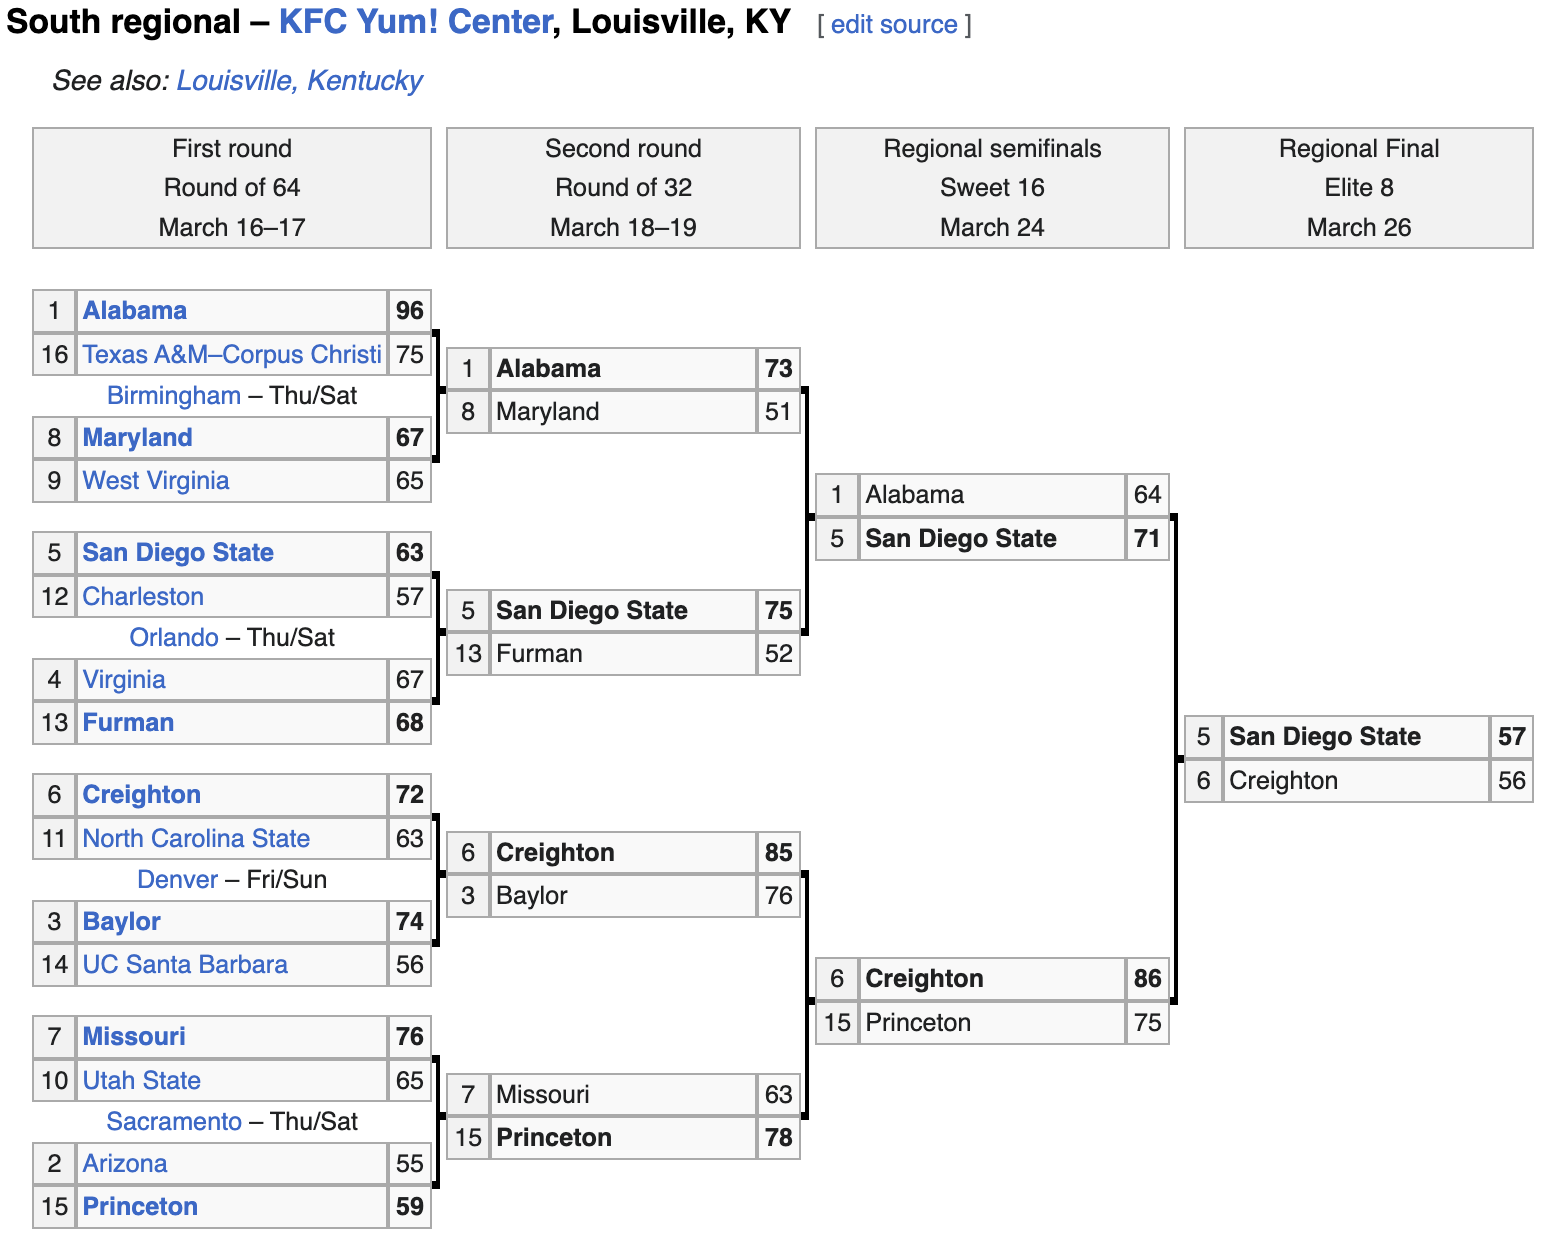
\includegraphics[width=\linewidth]{2023bracket}
\caption{\label{fig:bracket}Tournament bracket}
\end{figure}
the source for this bracket is
\begin{lstlisting}[basicstyle=\scriptsize,breaklines=true]
...
| RD1-seed01=1
| RD1-team01= '''[[2022-23 Alabama Crimson Tide men's basketball team|Alabama]]'''
| RD1-score01='''96'''
| RD1-seed02=16
| RD1-team02= [[2022-23 Texas A&M-Corpus Christi Islanders men's basketball team|Texas A&M-Corpus Christi]]
| RD1-score02=75
 
| RD1-seed03=8
| RD1-team03= '''[[2022-23 Maryland Terrapins men's basketball team|Maryland]]'''
| RD1-score03='''67'''
| RD1-seed04=9
| RD1-team04= [[2022-23 West Virginia Mountaineers men's basketball team|West Virginia]]
| RD1-score04=65
 
| RD1-seed05=5
| RD1-team05= '''[[2022-23 San Diego State Aztecs men's basketball team|San Diego State]]'''
| RD1-score05='''63'''
| RD1-seed06=12
| RD1-team06= [[2022-23 College of Charleston Cougars men's basketball team|Charleston]]
| RD1-score06=57
 
| RD1-seed07=4
| RD1-team07=[[2022-23 Virginia Cavaliers men's basketball team|Virginia]]
| RD1-score07=67
| RD1-seed08= 13
| RD1-team08= '''[[2022-23 Furman Paladins men's basketball team|Furman]]'''
| RD1-score08='''68'''
...
\end{lstlisting}
Each line begins with ``\texttt{| RD\#-[seed|team|score]\#\#}'', where the first number indicates the round, and the second numbers the teams within that round; teams numbered $2n-1$ and $2n$ will play each other.  Combining these results, we determine how often teams with a given seeding are victorious in 2766 (men's tournament) and 2309 (women's tournament) games through the year 2023. %, as shown in \autoref{tab:mD1_WL_prob}.
%\begin{table}
%\caption{\label{tab:mD1_WL_prob}Percent of matches that a team seeded \emph{row} defeated a team seeded \emph{columns} worse.}
%\tiny
%\begin{tabular}{ r *{15}{S[table-format=.2]} }\toprule
%\input{../bbm/D1/winlossprobs}
%\end{tabular}
%\end{table}
In \autoref{fig:D1_WL_prob}, we plot the fraction of games that the favored team wins as a function of the seed differential, along with their 95\% confidence intervals (using the Wilson interval\cite{Brown}).  We also plot the logistic best fits (determined using Python's Scikit\cite{scikit-learn}) $(1+\exp(-\beta x))^{-1}$ for $\beta=0.161$ (men's) and $\beta=0.276$ (women's).
\begin{figure}
\subcaptionbox{\label{fig:mD1_WL_prob}Men's. $\beta=0.161$}[.48\textwidth]{%
\begin{tikzpicture}
\begin{axis}[width=\linewidth,height=\linewidth,xmin=0,xmax=15.1,ymin=0,ymax=1,xlabel={Seed differential},ylabel={Fraction won by favored},axis y line=left,y axis line style=-,ticklabel style={font=\small}]
\addplot[dots](0,.5);
\addplot[domain=0:15]{1/(1+exp(-.161*x))};
\input{../bbm/D1/winlossplot}
\end{axis}
\end{tikzpicture}%
}\hfill
\subcaptionbox{\label{fig:wD1_WL_prob}Women's. $\beta=0.276$}[.48\textwidth]{%
\begin{tikzpicture}
\begin{axis}[width=\linewidth,height=\linewidth,xmin=0,xmax=15.1,ymin=0,ymax=1,xlabel={Seed differential},ylabel={Fraction won by favored},axis y line=left,y axis line style=-,ticklabel style={font=\small}]
\addplot[dots](0,.5);
\addplot[domain=0:15]{1/(1+exp(-.276*x))};
\input{../bbw/D1/winlossplot}
\end{axis}
\end{tikzpicture}
}
\caption{\label{fig:D1_WL_prob}Seed differential versus fraction of games that a favored team wins in the NCAA Division I basketball tournament, with 95\% Wilson confidence intervals and the logistic best fit.  Identical seed differentials have been slightly spread to avoid overlap.}
\end{figure}
Because a win for a given seed differential corresponds to a loss for that negated seed differential, the logistic curves are symmetric about $(0,0.5)$, and we only plot the curve for nonnegative seed differentials.  The confidence intervals do not inspire much confidence in this best fit, but we will be able to add more data as we proceed with our analysis.

A $\beta$ that is 70\% larger in the women's tournament than the men's tournament indicates that dramatic upsets are much less likely to occur.  In the men's tournament, upsets with a seed differential of 7 or more occurred 225 times out of 1225 games, or 18\% of the time.
% men upset: 31+38+47+45+58+2+4 = 225, men non upset: 328+195+180+150+126+15+3+1+2 = 1000
In the women's tournament, upsets with a seed differential of 7 or more occurred 76 times out of 928 games, or 8\% of the time.
% women upset: 9+8+16+11+32 = 76, women non upset: 282+174+150+134+111+1 = 852
A Fisher test shows that such upsets are more likely in the men's tournament ($p=\num{3.8e-12}$).

With $\beta=0.276$ and $p(x)=(1+\exp(-\beta x))^{-1}$, we are able to perform a calculation from the introduction.  The probability $P$ that there are no upsets in the first round of the women's tournament is $\prod_{i=1}^8 p(2i-1)^4\approx0.29\%$. The probability that the only upset is a single seed $k$ (losing to a seed $17-k$) is $P\cdot p(17-2k)^{-4}\cdot4p(17-2k)^3(1-p(17-2k))=4P\cdot(1-p(17-2k))/p(17-2k)$.  Therefore, the probability that there is at most one upset in the first round is
\[P+\sum_{k=1}^8 4P\frac{1-p(17-2k)}{p(17-2k)}\approx2.4\%.\]

We are interested in the question of how a team performs in a game after an upset win.  Are they tired from having over-exerted themselves, more experienced from having won a tournament game, or better than previously appreciated because we can now condition on them beating a supposedly superior opponent?  As %summarized in \autoref{tab:round_from_seeds} and
shown in \cite{Seltzer}, seed pairings must appear in known rounds.
%\begin{table}
%\caption{\label{tab:round_from_seeds}Round where seed of row and column must meet.  Entries on the main diagonal cannot meet.  All other meetings must occur in round 4.}
%\begin{tabular}{ r @{\qquad} *{16}r }\toprule
%  & 1 & 2 & 3 & 4 & 5 & 6 & 7 & 8 & 9 & 10 & 11 & 12 & 13 & 14 & 15 & 16 \\\cmidrule{2-17}
%1 & & & & 3 & 3 & & & 2 & 2 & & & 3 & 3 & & & 1\\
%2 & & & 3 & & & 3 & 2 & & & 2 & 3 & & & 3 & 1\\
%3 & & 3 & & & & 2 & 3 & & & 3 & 2 & & & 1 & 3\\
%4 & 3 & & & & 2 & & & 3 & 3 & & & 2 & 1 & & & 3\\
%5 & 3 & & & 2 & & & & 3 & 3 & & & 1 & 2 & & & 3\\
%6 & & 3 & 2 & & & & 3 & & & 3 & 1 & & & 2 & 3\\
%7 & & 2 & 3 & & & 3 & & & & 1 & 3 & & & 3 & 2\\
%8 & 2 & & & 3 & 3 & & & & 1 & & & 3 & 3 & & & 2\\
%9 & 2 & & & 3 & 3 & & & 1 & & & & 3 & 3 & & & 2\\
%10 & & 2 & 3 & & & 3 & 1 & & & & 3 & & & 3 & 2\\
%11 & & 3 & 2 & & & 1 & 3 & & & 3 & & & & 2 & 3\\
%12 & 3 & & & 2 & 1 & & & 3 & 3 & & & & 2 & & & 3\\
%13 & 3 & & & 1 & 2 & & & 3 & 3 & & & 2 & & & & 3\\
%14 & & 3 & 1 & & & 2 & 3 & & & 3 & 2 & & & & 3\\
%15 & & 1 & 3 & & & 3 & 2 & & & 2 & 3 & & & 3\\
%16 & 1 & & & 3 & 3 & & & 2 & 2 & & & 3 & 3\\\bottomrule
%\end{tabular}
%\end{table}
The seeds must add to 17 if and only if the teams meet in round one.  Teams meet in the second round if and only if the seeds add to 9 or 25 or differ by 8 (corresponding to 0, 2, or 1 upsets in the first round).
% x+y=9
% (17-x)+y=9
% x-y=8
% (17-x)+(17-y)=9
% 34-x-y=9
% 25=x+y
In \autoref{tab:D1_WL_prob_upset}, we examine the intervals from \autoref{fig:D1_WL_prob} that correspond to the second round after one first round upset.  The fraction of wins is slightly more in favor of an upset, but not significantly so.
\begin{table}\caption{\label{tab:D1_WL_prob_upset}Fraction of time that the better team wins in the second round, after one first round upset.  (Minimum 10 games.)}
\centering
\newbox\menswidest
\setbox\menswidest=\hbox{$69\pm15$}
\newbox\womenswidest
\setbox\womenswidest=\hbox{$68\pm13$}
\begin{tabular}{ c *2{S[table-format=2(2), uncertainty-mode=separate]} }\toprule
Seeds & {Men's (\%)} & {Women's (\%)} \\\midrule
1 v \phantom19 & 89(6) & 93(5) \\
2 v 10 & 62(12) & 84(9) \\
3 v 11 & 66(12) & 68(13) \\
4 v 12 & 69(13) & 82(13) \\
5 v 13 & 79(15) \\
6 v 14 & 80(16) \\\addlinespace
overall & 75(5) & 84(5)\\
\autoref{fig:D1_WL_prob} prediction & {\makebox[\wd\menswidest][l]{78.4}} & {\makebox[\wd\womenswidest][l]{90.1}} \\\bottomrule
\end{tabular}
\end{table}
%In \autoref{fig:D1_WL_prob_upset}, we plot the intervals from \autoref{fig:D1_WL_prob} that correspond to the second round after one first round upset in the men's (left) and women's (right) tournaments, along with logistic regressions for this filtered data.
%\begin{figure}
%\subcaptionbox{\label{fig:mD1_WL_prob_upset}Men's. $\beta=0.140$}[.48\textwidth]{%
%\begin{tikzpicture}
%\begin{axis}[width=\linewidth,height=\linewidth,xmin=0,xmax=15.1,ymin=0,ymax=1,xlabel={Seed differential},ylabel={Fraction won by favored},axis y line=left,y axis line style=-,ticklabel style={font=\small}]
%\addplot[dots](0,.5);
%\addplot[domain=0:15]{1/(1+exp(-.136*x))};
%% analyze.write_plot_file_round('bbm/D1/winloss.csv','bbm/D1/winlossRd2.tex',lambda r,c:c-r!=8)
%\input{../bbm/D1/winlossRd2}
%\end{axis}
%\end{tikzpicture}%
%}\hfill
%\subcaptionbox{\label{fig:wD1_WL_prob_upset}Women's. $\beta=0.218$}[.48\textwidth]{%
%\begin{tikzpicture}
%\begin{axis}[width=\linewidth,height=\linewidth,xmin=0,xmax=15.1,ymin=0,ymax=1,xlabel={Seed differential},ylabel={Fraction won by favored},axis y line=left,y axis line style=-,ticklabel style={font=\small}]
%\addplot[dots](0,.5);
%\addplot[domain=0:15]{1/(1+exp(-.218*x))};
%% analyze.write_plot_file_round('bbw/D1/winloss.csv','bbw/D1/winlossRd2.tex',lambda r,c:c-r!=8)
%\input{../bbw/D1/winlossRd2}
%\end{axis}
%\end{tikzpicture}
%}
%\caption{\label{fig:D1_WL_prob_upset}Seed differential versus fraction of games that a favored team wins in their tournament in the second round after one first round upset, with 95\% Wilson confidence intervals and the logistic best fit.}
%\end{figure}
%The smaller value of $\beta$ does indicate that an upset is more likely to occur again.

In 2001, the men's tournament added a ``play-in'' game, where the last two teams to make the tournament played each other for the last spot.  (The NCAA initially referred to this as the first round, but later branded this the ``First Four'' so that ``first round'' would still refer to the round with 64 teams.  We use the ``later'' terminology.)  The play-in game expanded to eight teams for four spots in 2011.  We are interested in the question of how the play-in winners perform in their first round game: are they tired from having played earlier in the week, more experienced from having played a tournament game, or better than previously appreciated because we can now condition on them beating a supposedly equivalent opponent?  We are able to identify play-in games by looking for identically high seeded teams.  We then record how the winning team performs in their first round game, and summarize according to their seed in \autoref{tab:play_in_subsequent}.
\begin{table}
\centering%\small
\caption{\label{tab:play_in_subsequent}Number of games won in first round in the men's tournament, by seed, where the worse seed was (not) the winner of a play-in game.  Also significance of the statement ``Play-in winners are more likely to have an upset in their first round.''}
\begin{tabular}{ @{} c *{10}{S[table-format=2]} *{2}{S[table-format=3]} @{} }\toprule
%& \multicolumn{10}c{By individual seed} \\\cmidrule(lr){2-11}\cmidrule(l){12-13}
Seed & {6} & 11 & {5} & 12 & {4} & 13 & {3} & 14 & {1} & 16 & \multicolumn2c{Overall} \\ %& 6 & 11 & 1 & 16 \\
\cmidrule(lr){2-3}\cmidrule(lr){4-5}\cmidrule(lr){6-7}\cmidrule(lr){8-9}\cmidrule(lr){10-11}\cmidrule(l){12-13}%\cmidrule(l){14-15}
Play-in & 9 & 9 & 3 & 1 & 0 & 1 & 1 & 0 & 33 & 1 & 46 & 12 \\ %3 & 1 & 4 & 0 \\
Non-play-in & 40 & 30 & 50 & 34 & 68 & 19 & 78 & 19 & 53 & 1 & 289 & 103 \\\addlinespace % 2 & 2 & 4 & 0 \\\addlinespace
$p$ & \multicolumn2c{0.39} & \multicolumn2c{0.87} & \multicolumn2c{0.23} & \multicolumn2c{1} & \multicolumn2c{0.63} & \multicolumn2c{0.86} %\multicolumn2c{0.93} & \multicolumn2c{1}
\\\bottomrule
\end{tabular}
\end{table}
Each seed has 88 total games from 22 years and 4 games per seed per year.  Of those 88, the first row of the table counts games played with play-in winners of that seed, while the second row counts games with non-play-in winners.  The left column of each pair counts games where the favored team won, while the right column counts upsets.  The final row gives the significance that play-in winners are more likely to have an upset.  Given the high $p$ values, we are unable to substantiate this claim.  There is even less data for the women's tournament, which has only had 8 play-in games since they were added in 2022.

Each year, the bracket's unveiling is met with inevitable second guessing that a team should be seeded differently.  Fans (and foes) of a particular team will often claim that team over (or under) performs in the tournament, or even that the team consistently receives (un)favorable bias from the selection committee.

We are able to examine these claims by recording how a team performs each year during the tournament.  But while collecting this data, we quickly run into a problem: the millions of Wikipedia editors (unsurprisingly) have not entered the team names consistently.  For example, eventually we see twelve of the twenty four possible configurations of S[o[uth[ern]]] Conn[ecticut] [St[ate]], only some of which use a period for the abbreviations, that should all become ``Southern Connecticut''.  Even within a single bracket (presumably one editor), a team tends to have a more abbreviated name in later rounds. We will therefore devote a large portion of our code to normalizing the team names that appear by expanding most abbreviations and dropping unnecessary words, occasionally resulting in a team name that is slightly different than what the media and fans customarily use.

Once team names have been normalized, we still have a problem of ambiguity.  We will convert ``USC'' to ``Southern California'' or ``South Carolina'', often by looking for which mascot appears elsewhere on the page (a conference is also helpful).  Similarly, ``Saint John's'' will become ``Saint John's New York'' or ``Saint John's Minnesota'' along with scores of other disambiguations.

Within our sample, UNC (now North Carolina) has played the most men's tournament games at 136, while (the University of) Tennessee has played the most women's tournament games at 163.  Plotting the seed differences of those games along with whether the game was a win (104 and 129 times) or a loss (32 and 34 times) along with the logistic regressions gives \autoref{fig:bbm_D1_team}.
\begin{figure}
\subcaptionbox{\label{fig:bbm_D1_UNC}North Carolina men. $\beta=0.192$}[.48\textwidth]{%
\begin{tikzpicture}
\begin{axis}[width=\linewidth,height=\linewidth,xmin=-16,xmax=16,ymin=0,ymax=1,axis y line=center,y axis line style=-,x axis line style=<->,xlabel={Seed differential},clip=false,xtick={-10,10},ticklabel style={font=\small},tickwidth=.3cm]
\addplot[domain=-15:15]{1/(1+exp(-.192*(x+2.78)))};
\addplot[dots](-2.78,.5)node[left]{\small$\mu=-2.78$};
\addplot[dots](8,1)node[above]{\tiny11};
\addplot[dots](3,1)node[below]{\tiny7};
\addplot[dots](2,1)node[above]{\tiny4};
\addplot[dots](5,1)node[below]{\tiny11};
\addplot[dots](0,1)node[above]{\tiny4};
\addplot[dots](1,1)node[below]{\tiny14};
\addplot[dots](7,1)node[below]{\tiny7};
\addplot[dots](13,1)node[below]{\tiny7};
\addplot[dots](9,1)node[below]{\tiny6};
\addplot[dots](11,1)node[below]{\tiny3};
\addplot[dots](15,1)node[below]{\tiny14};
\addplot[dots](4,1)node[above]{\tiny7};
\addplot[dots](-7,1)node[below]{\tiny3};
\addplot[dots](-1,1)node[below]{\tiny2};
\addplot[dots](-4,1)node[above]{\tiny2};
\addplot[dots](12,1)node[above]{\tiny1};
\addplot[dots](-6,1)node[above]{\tiny1};
\addplot[dots](2,0)node[below]{\tiny4};
\addplot[dots](3,0)node[above]{\tiny2};
\addplot[dots](6,0)node[below]{\tiny1};
\addplot[dots](-1,0)node[above]{\tiny2};
\addplot[dots](1,0)node[above]{\tiny6};
\addplot[dots](-4,0)node[below]{\tiny1};
\addplot[dots](-3,0)node[above]{\tiny6};
\addplot[dots](8,0)node[below]{\tiny2};
\addplot[dots](0,0)node[below]{\tiny2};
\addplot[dots](11,0)node[above]{\tiny1};
\addplot[dots](5,0)node[above]{\tiny2};
\addplot[dots](-7,0)node[above]{\tiny2};
\addplot[dots](4,0)node[below]{\tiny1};
\end{axis}
\end{tikzpicture}%
}\hfill
\subcaptionbox{\label{fig:bbw_D1_Tenn}Tennessee women. $\beta=0.304$}[.48\textwidth]{%
\begin{tikzpicture}
\begin{axis}[width=\linewidth,height=\linewidth,xmin=-16,xmax=16,ymin=0,ymax=1,axis y line=center,y axis line style=-,x axis line style=<->,xlabel={Seed differential},clip=false,xtick={-10,10},ticklabel style={font=\small},tickwidth=.3cm]
\addplot[domain=-15:15]{1/(1+exp(-.304*(x+1.92)))};
\addplot[dots](-1.92,.5)node[left]{\small$\mu=-1.92$};
\addplot[dots](5,1)node[below]{\tiny6};
\addplot[dots](1,1)node[below]{\tiny13};
\addplot[dots](-1,1)node[below]{\tiny7};
\addplot[dots](7,1)node[below]{\tiny14};
\addplot[dots](3,1)node[below]{\tiny18};
\addplot[dots](-2,1)node[above]{\tiny4};
\addplot[dots](0,1)node[above]{\tiny10};
\addplot[dots](-3,1)node[below]{\tiny1};
\addplot[dots](8,1)node[above]{\tiny14};
\addplot[dots](4,1)node[above]{\tiny4};
\addplot[dots](2,1)node[above]{\tiny6};
\addplot[dots](15,1)node[below]{\tiny15};
\addplot[dots](11,1)node[below]{\tiny3};
\addplot[dots](13,1)node[below]{\tiny5};
\addplot[dots](9,1)node[below]{\tiny5};
\addplot[dots](12,1)node[above]{\tiny1};
\addplot[dots](6,1)node[above]{\tiny1};
\addplot[dots](-5,1)node[below]{\tiny1};
\addplot[dots](-4,1)node[above]{\tiny1};
\addplot[dots](-1,0)node[above]{\tiny7};
\addplot[dots](3,0)node[above]{\tiny9};
\addplot[dots](1,0)node[above]{\tiny6};
\addplot[dots](-2,0)node[below]{\tiny1};
\addplot[dots](-3,0)node[above]{\tiny4};
\addplot[dots](0,0)node[below]{\tiny4};
\addplot[dots](2,0)node[below]{\tiny1};
\addplot[dots](7,0)node[above]{\tiny1};
\addplot[dots](-5,0)node[above]{\tiny1};
\end{axis}
\end{tikzpicture}
}
\caption{\label{fig:bbm_D1_team}Wins and losses (with multiplicity) in the NCAA Division I basketball tournament, along with the logistic regression $(1+\exp(-\beta(x-\mu)))^{-1}$.}
\end{figure}

The logistic function $(1+\exp(-\beta(x-\mu)))^{-1}$ for $\beta=0.192$ and $\mu=2.78$ suggests that UNC performs about 2.78 seedings worse than expected, while $\beta=0.304$ and $\mu=1.92$ suggests that Tennessee performs about 1.92 seedings worse.  The larger $\beta$ also indicates that Tennessee is more likely to avoid an upset (for better and worse).

Of the 313 (299) teams that have participated in the men's (women's) tournament, 131 (110) have at least 10 games in the tournament and at least 1 win.  Of these, only 7 men's (1 women's) teams have $\beta<0.01$, causing a large $\mu$.  Repeating the calculation of $\mu$ for the remaining 124 (109) teams and plotting the number of games along with the team's $\mu$ gives us \autoref{fig:bb_D1_game_v_mu}.
%\begin{figure}
%\subcaptionbox{\label{fig:bbm_D1_game_v_mu}Rate versus expected reseeding in the men's tournament.}[.48\textwidth]{
%\begin{tikzpicture}
%\begin{axis}[width=\linewidth,height=\linewidth,axis y line=left,axis x line=center,y axis line style=<->,xmin=-.2,xmax=1.4,ymin=-10,ymax=10,xlabel={Rate $\beta$},ylabel={Expected reseeding $\mu$}]
% \csvreader[head to column names, filter fp = {\Games>9 && \Reseed!=16}]
%   {../bbm/D1/reseed.csv}{}{\addplot[dots](\Rate,\Reseed);}
%\end{axis}
%\end{tikzpicture}
%}\hfill
%\subcaptionbox{\label{fig:bbw_D1_game_v_mu}Rate versus expected reseeding in the women's tournament.}[.48\textwidth]{
%\begin{tikzpicture}
%\begin{axis}[width=\linewidth,height=\linewidth,axis y line=left,axis x line=center,y axis line style=<->,xmin=-.2,xmax=1.4,ymin=-10,ymax=10,xlabel={Rate $\beta$},ylabel={Expected reseeding $\mu$}]
% \csvreader[head to column names, filter fp = {\Games>9 && \Reseed!=16}] %  && \Reseed<10 && -10<\Reseed
%   {../bbw/D1/reseed.csv}{}{\addplot[dots](\Rate,\Reseed);}
%\end{axis}
%\end{tikzpicture}
%}
%\end{figure}

\begin{figure}
\subcaptionbox{\label{fig:bbm_D1_game_v_mu}Men's}[.48\textwidth]{%
\begin{tikzpicture}
\begin{axis}[width=\linewidth,height=.8\linewidth,axis y line=left,axis x line=center,y axis line style=<->,
	xmin=9.1,xmax=170,ymin=-10,ymax=10,xmode=log,xtick={10,20,50,100},xticklabels={10,20,50,100},xlabel={\# Games},ylabel={Expected reseeding},
	ticklabel style={font=\small},tickwidth=.3cm,restrict y to domain=-10:10]
 \addplot[dots] table[col sep=comma,x=Games,y=Reseed,only marks]{../bbm/D1/reseed.csv};
% \csvreader[head to column names, filter fp = {\Games>9 && \Rate>0.01}]
%   {../bbm/D1/reseed.csv}{}{\addplot[dots](\Games,\Reseed);}
\end{axis}
\end{tikzpicture}
}\hfill
\subcaptionbox{\label{fig:bbw_D1_game_v_mu}Women's}[.48\textwidth]{%
\begin{tikzpicture}
\begin{axis}[width=\linewidth,height=.8\linewidth,axis y line=left,axis x line=center,y axis line style=<->,
	xmin=9.1,xmax=170,ymin=-10,ymax=10,xmode=log,xtick={10,20,50,100},xticklabels={10,20,50,100},xlabel={\# Games},ylabel={Expected reseeding},
	ticklabel style={font=\small},tickwidth=.3cm,restrict y to domain=-10:10]
 \addplot[dots] table[col sep=comma,x=Games,y=Reseed,only marks]{../bbw/D1/reseed.csv};
% \csvreader[head to column names, filter fp = {\Games>9 && \Rate>0.01}]
%   {../bbw/D1/reseed.csv}{}{\addplot[dots](\Games,\Reseed);}
\end{axis}
\end{tikzpicture}
}
\caption{\label{fig:bb_D1_game_v_mu}(Logarithmic) number of games versus expected reseeding in each NCAA Division I basketball tournament.}
\end{figure}
We observe a slight negative trend of reseeding for the teams that have a large number of games (the right most four men's teams are perennial contenders Kentucky, Kansas, Duke, and North Carolina, while the right three women's teams are Stanford, Connecticut, and Tennessee).
Such teams have a large amount of victories against lower ranking teams, so that the logistic best fit is pulled up and toward a negative $\mu$.
% on the other hand, we can also say:
%  Teams that have a favorable seeding rarely play a better seed, and are therefore unable to show that they should have been even more favorably seeded. Consequently, the occasional upset they experience causes their expected reseeding to be worse.
% so we can argue either way, which isn't great

Having failed to identify any bias for or against a particular team, we consider the possibility that a \emph{group} of teams may experience some bias.  We repeat the calculation of $\mu$, now grouping teams by their state in \autoref{fig:bb_D1_game_v_mu_by_state} and (slightly inaccurately) grouping the states by timezone in \autoref{fig:bb_D1_game_v_mu_by_timezone}.
\begin{figure}
\subcaptionbox{\label{fig:bbm_D1_game_v_mu_by_state}Men's, omitting DE (0-7); HI (1-4); ND (2-5); SD (0-6); AK, ME, NH (all 0-0).}[.48\textwidth]{%
\begin{tikzpicture}
\begin{axis}[width=\linewidth,height=.8\linewidth,axis y line=left,axis x line=center,y axis line style=<->,
	xmin=9.1,xmax=450,ymin=-10,ymax=10,xmode=log,xtick={10,20,50,100,200},xticklabels={10,20,50,100,200},
	xlabel={\# Games},ylabel={Expected reseeding},
	ticklabel style={font=\small},tickwidth=.3cm,xlabel style={yshift=-7ex},restrict y to domain=-10:10]
 \addplot[dots] table[col sep=comma,x=Games,y=Reseed,only marks]{../bbm/D1/state_reseed.csv};
% \csvreader[head to column names, filter fp = {\Games>9 && \Rate>0.01}]
%   {../bbm/D1/state_reseed.csv}{}{\addplot[dots](\Games,\Reseed);}
\end{axis}
\end{tikzpicture}
}\hfill
\subcaptionbox{\label{fig:bbw_D1_game_v_mu_by_state}Women's, omitting AK (0-0), DE (3-6), HI (1-8), ID (0-14), NH (0-7), ND (0-1), RI (2-7), VT (1-7), WY (0-2).}[.48\textwidth]{%
\begin{tikzpicture}
\begin{axis}[width=\linewidth,height=.8\linewidth,axis y line=left,axis x line=center,y axis line style=<->,
	xmin=9.1,xmax=450,ymin=-10,ymax=10,xmode=log,xtick={10,20,50,100,200},xticklabels={10,20,50,100,200},
	xlabel={\# Games},ylabel={Expected reseeding},
	ticklabel style={font=\small},tickwidth=.3cm,xlabel style={yshift=-7ex},restrict y to domain=-10:10]
 \addplot[dots] table[col sep=comma,x=Games,y=Reseed,only marks]{../bbw/D1/state_reseed.csv};
% \csvreader[head to column names, filter fp = {\Games>9 && \Rate>0.01}]
%   {../bbw/D1/state_reseed.csv}{}{\addplot[dots](\Games,\Reseed);}
\end{axis}
\end{tikzpicture}
}
\caption{\label{fig:bb_D1_game_v_mu_by_state}(Logarithmic) number of games versus expected reseeding in each NCAA Division I basketball tournament, grouped by state.}
\end{figure}
%
\begin{figure}
\subcaptionbox{\label{fig:bbm_D1_game_v_mu_by_timezone}Men's, omitting Alaska (0-0) and Hawaii (1-4).}[.48\textwidth]{%
\begin{tikzpicture}
\begin{axis}[width=\linewidth,height=.8\linewidth,axis y line=left,axis x line=center,y axis line style=<->,
	xmin=100,xmax=3200,ymin=-2,ymax=3,xmode=log,xtick={100,200,500,1000,2000},xticklabels={100,200,500,1000,2000},
	xlabel={\# Games},ylabel={Expected reseeding},nodes near coords,point meta=explicit symbolic,mark size=2pt,
	ticklabel style={font=\small},tickwidth=.3cm,restrict y to domain=-10:10,coordinate style/.condition={-.8<y&&y<-.5}{below}] % ,xlabel style={yshift=-7ex}
 \addplot[dots] table[col sep=comma,x=Games,y=Reseed,meta=Team,only marks]{../bbm/D1/tz_reseed.csv};
% \csvreader[head to column names, filter fp = {\Games>9 && \Rate>0.01}]
%   {../bbm/D1/state_reseed.csv}{}{\addplot[dots](\Games,\Reseed);}
\end{axis}
\end{tikzpicture}
}\hfill
\subcaptionbox{\label{fig:bbw_D1_game_v_mu_by_timezone}Women's, omitting Alaska (0-0) and Hawaii (1-8).}[.48\textwidth]{%
\begin{tikzpicture}
\begin{axis}[width=\linewidth,height=.8\linewidth,axis y line=left,axis x line=center,y axis line style=<->,
	xmin=100,xmax=3200,ymin=-2,ymax=3,xmode=log,xtick={100,200,500,1000,2000},xticklabels={100,200,500,1000,2000},
	xlabel={\# Games},ylabel={Expected reseeding},nodes near coords,point meta=explicit symbolic,mark size=2pt,
	ticklabel style={font=\small},tickwidth=.3cm,xlabel style={yshift=-7ex},restrict y to domain=-10:10,
	coordinate style/.condition={-.8<y&&y<-.5}{below}
	]
 \addplot[dots] table[col sep=comma,x=Games,y=Reseed,meta=Team,only marks]{../bbw/D1/tz_reseed.csv};
% \csvreader[head to column names, filter fp = {\Games>9 && \Rate>0.01}]
%   {../bbw/D1/state_reseed.csv}{}{\addplot[dots](\Games,\Reseed);}
\end{axis}
\end{tikzpicture}
}
\caption{\label{fig:bb_D1_game_v_mu_by_timezone}(Logarithmic) number of games versus expected reseeding in each NCAA Division I basketball tournament, grouped by timezone.}
\end{figure}
For the timezone plot, note that we include Arizona (Mountain Standard Time) in Mountain (Daylight) Time because the majority of the college season occurs outside of Daylight Saving Time.  Also, we include Indiana in Eastern Time. % because Indiana and timezones are just confusing.

We now focus on our original example, that an 11 seed won games with seed differentials $-5$, $3$, $-9$, and $-7$.  For a game with seed differential $s$, we previously approximated the probability of the favored team winning by $p(s)=(1+\exp(-\beta s))^{-1}$, where $\beta=0.161$ for this tournament.  Treating these as four independent games would give a probability of $0.89\%$. We will instead argue that the upsets in rounds 1 and 3 indicate that the team should have been seeded better, making the victories in rounds 2--4 and then round 4 more likely.

Returning to the 124 men's (109 women's) teams, if we discard 3 (1) outliers where $\lvert\mu\rvert>16$, then we can weight the remaining 121 (108) values of $\mu$ by the number of games the team played to estimate that $\mu$ has a mean $\mu_0$  of $-0.2$ (0.15) and a standard deviation $\sigma$  of 3.2 (2.1). This means that we can instead assume that a better seeded team is correctly seeded, and that a worse seeded team should have had their seed adjusted downward by the appropriate normal random variable $X$.  In that case, the most likely seeding correction in the event of an upset would be the maximizer of
\[\frac1{\sigma\sqrt{2\pi}}\exp\Bigl\{-\frac{(X-\mu_0)^2}{2\sigma^2}\Bigr\}\frac{\exp(-\beta(s-X))}{1+\exp(-\beta(s-X))}.\]
This maximum occurs at the root of the nonlinear equation
\[\frac\beta{1+\exp(-\beta(s-X))}=\frac{X-\mu_0}{\sigma^2}.\]
With our values of $\beta$, $\mu_0$, and $\sigma$, a numerical solver estimates that on $1\le s\le15$, this root is approximately $0.68+\frac s{25}$ for the men's tournament and $0.89+\frac s{33}$ for the women's tournament.  This means that after an 11 seed defeats a 6 seed, we should instead model the 11 seed as if they had been seeded 10.12.  Treating the last three games dependent on the first one (but independent from each other), we would act as if the seed differentials had be $-5$, $3.88$, $-8.12$, and $-6.12$, bringing the probability up to $1.2\%$.

Repeating this analysis for two upsets, we would want to maximize
\[
\frac1{\sigma\sqrt{2\pi}}\exp\Bigl\{-\frac{(X-\mu_0)^2}{2\sigma^2}\Bigr\}
\frac{\exp(-\beta(s_1-X))}{1+\exp(-\beta(s_1-X))}
\frac{\exp(-\beta(s_2-X))}{1+\exp(-\beta(s_2-X))},
\]
which happens when
\[\frac\beta{1+\exp(-\beta(s_1-X))}+\frac\beta{1+\exp(-\beta(s_2-X))}=\frac{X-\mu_0}{\sigma^2}.\]
This root is approximately $1.43+\frac{s_1+s_2}{24}$ for the men (and $1.48+\frac{s_1+s_2}{29}$ for the women) on $1\le s_1,s_2\le15$, so that after upsets of seed differentials $-5$ and $-9$, we should instead model the 11 seed as if they had been seeded 9.  Repeating our calculation with seed differentials of $-5$, $3.88$, $-8.12$, and $-5$, the probability is now the previously stated $1.3\%$.

We will now revisit the probability of an upset in the second round after an upset in the first, examined in light of reseeding.  For a logistic function $p(s)=(1+\exp(-\beta_0-\beta_1s))^{-1}$, the log-likelihood $\ell$ is the expression $Y_k\ln p(S_k)+(1-Y_k)\ln(1-p(S_k))$ where $S_k$ is the seed differential (positive for a favored team) and $Y_k$ is 1 in victory and 0 in defeat.  The expression is maximized when $p$ is the logistic best fit (note that this logistic function is slightly different than ours, where $\beta=\beta_1$ and $\mu=-\beta_0/\beta_1$, although $\mu=\beta_0=0$ because of symmetry in our case).  In \autoref{tab:D1_log_likely_upset}, we see the average log-likelihood for each second round matchup after a first round upset.
\begin{table}\caption{\label{tab:D1_log_likely_upset}Average log-likelihood in the second round, after one first round upset, with and without reseeding.  (Minimum 10 games.)}
\centering
\begin{tabular}{ c *4{S[table-format=-1.2]} }\toprule
\multirow{2}{*}{Seeds} & \multicolumn2c{Men's} & \multicolumn2c{Women's} \\
 & {Without} & {With} & {Without} & {With} \\\midrule
1 v \phantom19 & -1.27 & -1.19 & -2.17 & -1.96 \\
2 v 10 & -0.49 & -0.44 & -1.86 & -1.69 \\
3 v 11 & -0.61 & -0.56 & -1.28 & -1.15 \\
4 v 12 & -0.71 & -0.67 & -1.84 & -1.69 \\
5 v 13 & -1.11 & -1.08 \\
6 v 14 & -1.18 & -1.16 \\\addlinespace
overall & -0.83 & -0.78 & -1.80 & -1.64 \\\bottomrule
\end{tabular}
\end{table}
Using the reseeding results in a better (less negative) average log-likelihood.


\section{College Basketball Tournaments}
Wikipedia has brackets for many other basketball tournaments, most notably 32 (32) different conference tournaments [with occasional changing names] determining a champion for an automatic bid to the men's (women's) national tournament.  There are also 7 (4) other tournaments with a national scope.  We again begin by plotting seed differential against fraction of games won by the favored team in \autoref{fig:bb_WL_prob},
\begin{figure}
\subcaptionbox{\label{fig:bbm_WL_prob}Men's. $\beta=0.202$}[.48\textwidth]{%
\begin{tikzpicture}
\begin{axis}[width=\linewidth,height=.8\linewidth,xmin=0,xmax=15.1,ymin=0,ymax=1,xlabel={Seed differential},ylabel={Fraction won by favored},axis y line=left,y axis line style=-]
\addplot[dots](0,.5);
\addplot[domain=0:15]{1/(1+exp(-.202*x))};
% analyze.analyze_winloss('bbm/winloss.csv')
\input{../bbm/winlossplot}
\end{axis}
\end{tikzpicture}
}\hfill
\subcaptionbox{\label{fig:bbw_WL_prob}Women's. $\beta=0.284$}[.48\textwidth]{%
\begin{tikzpicture}
\begin{axis}[width=\linewidth,height=.8\linewidth,xmin=0,xmax=15.1,ymin=0,ymax=1,xlabel={Seed differential},ylabel={Fraction won by favored},axis y line=left,y axis line style=-]
\addplot[dots](0,.5);
\addplot[domain=0:15]{1/(1+exp(-.284*x))};
% analyze.analyze_winloss('bbw/winloss.csv')
\input{../bbw/winlossplot}
\end{axis}
\end{tikzpicture}
}
\caption{\label{fig:bb_WL_prob}Seed differential versus fraction of games that a favored team wins in basketball tournaments, with 95\% Wilson confidence intervals and the logistic best fit.}
\end{figure}
and then the number of games compared to how a team should be reseeded in \autoref{fig:bb_game_v_mu}.
\begin{figure}
\subcaptionbox{\label{fig:bbm_game_v_mu}Men's}[.48\textwidth]{%
\begin{tikzpicture}
\begin{axis}[width=\linewidth,height=.8\linewidth,axis y line=left,axis x line=center,y axis line style=<->,
  xmin=9.1,xmax=320,ymin=-10,ymax=10,xmode=log,xtick={10,20,50,100,200},xticklabels={10,20,50,100,200},xlabel style={yshift=-7ex},
  xlabel={\# of games},ylabel={Expected reseeding}]
 \addplot[dots] table[col sep=comma,x=Games,y=Reseed,only marks]{../bbm/reseed_filtered.csv};
\end{axis}
\end{tikzpicture}
}\hfill
\subcaptionbox{\label{fig:bbw_game_v_mu}Women's}[.48\textwidth]{%
\begin{tikzpicture}
\begin{axis}[width=\linewidth,height=.8\linewidth,axis y line=left,axis x line=center,y axis line style=<->,
  xmin=9.1,xmax=320,ymin=-10,ymax=10,xmode=log,xtick={10,20,50,100,200},xticklabels={10,20,50,100,200},xlabel style={yshift=-7ex},
  xlabel={\# of games},ylabel={Expected reseeding}]
 \addplot[dots] table[col sep=comma,x=Games,y=Reseed,only marks]{../bbw/reseed_filtered.csv};
\end{axis}
\end{tikzpicture}
}
\caption{\label{fig:bb_game_v_mu}(Logarithmic) number of games versus expected reseeding in basketball tournaments.}
\end{figure}

We also summarize the likelihood of upsets by calculating $\beta$ for each tournament, and plot the results in \autoref{fig:bb_game_v_rate}.
\begin{figure}
\subcaptionbox{\label{fig:bbm_game_v_rate}Men's}[.48\textwidth]{%
\begin{tikzpicture}
\pgfplotstableread[col sep=comma]{../bbm/group_betas.csv}\datatable
\begin{axis}[width=\linewidth,height=.8\linewidth,axis y line=left,axis x line=center,y axis line style=->,
  xmin=20,xmax=3000,ymin=0,ymax=.8,xmode=log,xtick={50,100,200,500,1000,2000},xticklabels={50,100,200,500,1k,2k},
  xlabel={\# of games},ylabel={$\beta$}]
 \addplot[scatter,only marks,draw=black,scatter/classes={0={mark=*,mark size=.5pt},1={mark=+,mark size=2pt}},
  scatter src=explicit symbolic] table[x=Games,y=Rate,meta=IsNational]\datatable;
\end{axis}
\end{tikzpicture}
}\hfill
\subcaptionbox{\label{fig:bbw_game_v_rate}Women's}[.48\textwidth]{%
\begin{tikzpicture}
\pgfplotstableread[col sep=comma]{../bbw/group_betas.csv}\datatable
\begin{axis}[width=\linewidth,height=.8\linewidth,axis y line=left,axis x line=center,y axis line style=->,
  xmin=20,xmax=3000,ymin=0,ymax=.8,xmode=log,xtick={50,100,200,500,1000,2000},xticklabels={50,100,200,500,1k,2k},
  xlabel={\# of games},ylabel={$\beta$}]
 \addplot[scatter,only marks,draw=black,scatter/classes={0={mark=*,mark size=.5pt},1={mark=+,mark size=2pt}},
  scatter src=explicit symbolic] table[x=Games,y=Rate,meta=IsNational]\datatable;
\end{axis}
\end{tikzpicture}
}
\caption{\label{fig:bb_game_v_rate}(Logarithmic) number of games versus upset rate in basketball tournaments. National tournaments denoted with +.}
\end{figure}
Note that national conferences generally have lower $\beta$ values, suggesting that upsets are more common.  Within a conference tournament, most teams have already played each other, and a team's record (which all conferences use for seeding) is a useful estimate of how good the team is.  In a national tournament, on the other hand, most teams have not played each other.  In this case, tournament organizers resort to (sometimes objective) arbitrary methods to determine seedings, but these methods are not as useful at estimating how good the teams are.

To examine one conference tournament slightly more in-depth, we plot in \autoref{fig:bb_sec_game_v_mu} the number of games versus the expected reseeding for the SEC, located at $(504,0.21)$ in \autoref{fig:bbm_game_v_rate} and $(240,0.29)$ in \autoref{fig:bbw_game_v_rate}.
\begin{figure}
\subcaptionbox{\label{fig:bbm_sec_game_v_mu}Men's}[.48\textwidth]{%
\begin{tikzpicture}
\begin{axis}[width=\linewidth,height=.8\linewidth,axis y line=left,axis x line=center,y axis line style=<->,
  xmin=9.1,xmax=150,ymin=-5,ymax=5,xmode=log,xtick={10,20,50,100},xticklabels={10,20,50,100},xlabel style={yshift=-7ex},
  xlabel={\# of games},ylabel={Expected reseeding}]
 \addplot[dots] table[col sep=comma,x=Games,y=Reseed,only marks]{../bbm/SEC/reseed.csv};
\end{axis}
\end{tikzpicture}
}\hfill
\subcaptionbox{\label{fig:bbw_sec_game_v_mu}Women's}[.48\textwidth]{%
\begin{tikzpicture}
\begin{axis}[width=\linewidth,height=.8\linewidth,axis y line=left,axis x line=center,y axis line style=<->,
  xmin=9.1,xmax=150,ymin=-5,ymax=5,xmode=log,xtick={10,20,50,100},xticklabels={10,20,50,100},xlabel style={yshift=-7ex},
  xlabel={\# of games},ylabel={Expected reseeding}]
 \addplot[dots] table[col sep=comma,x=Games,y=Reseed,only marks]{../bbw/SEC/reseed.csv};
\end{axis}
\end{tikzpicture}
}
\caption{\label{fig:bb_sec_game_v_mu}(Logarithmic) number of games versus expected reseeding in SEC basketball tournaments.}
\end{figure}
We again observe a negative reseeding bias for teams that have played the most games (Kentucky for the men and Tennessee for the women).  This bias cannot be blamed on non-existent selection committees.

We would like to calculate conferences' expected reseeding to compare how conferences have performed in national tournaments over the years.  Unfortunately, the teams in a conference have shifted, so that we cannot make a simple list of which teams go to which conference.  Instead, for a particular year we will note which teams participated in which conference tournaments.  Then in national tournaments we will record how conferences performed against each other in \autoref{fig:bb_conf_game_v_mu}.
\begin{figure}
\subcaptionbox{\label{fig:bbm_conf_game_v_mu}Men's}[.48\textwidth]{%
\begin{tikzpicture}
\pgfplotstableread[col sep=comma]{../bbm/conf_reseed.csv}\datatable
\begin{axis}[width=\linewidth,height=.8\linewidth,axis y line=left,axis x line=center,y axis line style=<->,
  xmin=9.1,xmax=1000,ymin=-10,ymax=10,xmode=log,xtick={10,20,50,100,200,500},xticklabels={10,20,50,100,200,500},xlabel style={yshift=-7ex},
  xlabel={\# of games},ylabel={Expected reseeding}]
 \addplot[scatter,only marks,draw=black,scatter/classes={0={mark=+,mark size=2pt},1={mark=*,mark size=.5pt}},
  scatter src=explicit symbolic] table[x=Games,y=Reseed,meta=ConferenceIsKnown]\datatable;
% \addplot[dots] table[col sep=comma,x=Games,y=Reseed,only marks]{../bbm/conf_reseed.csv};
% \addplot[black,mark=+,mark size=2pt](649,-0.766035771331451);  % can I automate "Conference == ''" ?
\end{axis}
\end{tikzpicture}
}\hfill
\subcaptionbox{\label{fig:bbw_conf_game_v_mu}Women's}[.48\textwidth]{%
\begin{tikzpicture}
\pgfplotstableread[col sep=comma]{../bbw/conf_reseed.csv}\datatable
\begin{axis}[width=\linewidth,height=.8\linewidth,axis y line=left,axis x line=center,y axis line style=<->,
  xmin=9.1,xmax=1000,ymin=-10,ymax=10,xmode=log,xtick={10,20,50,100,200,500},xticklabels={10,20,50,100,200,500},xlabel style={yshift=-7ex},
  xlabel={\# of games},ylabel={Expected reseeding}]
 \addplot[scatter,only marks,draw=black,scatter/classes={0={mark=+,mark size=2pt},1={mark=*,mark size=.5pt}},
  scatter src=explicit symbolic] table[x=Games,y=Reseed,meta=ConferenceIsKnown]\datatable;
% \addplot[dots] table[col sep=comma,x=Games,y=Reseed,only marks]{../bbw/conf_reseed.csv};
% \addplot[black,mark=+,mark size=2pt](494,-0.156496429184286);  % ditto
\end{axis}
\end{tikzpicture}
}
\caption{\label{fig:bb_conf_game_v_mu}(Logarithmic) number of games versus expected reseeding of conferences in national basketball tournaments.  Unknown conferences have been consolidated into +.}
\end{figure}


%\section{College Tournaments}
Wikipedia has many more tournaments to analyze.  We tabulate the collegiate tournaments in \autoref{tab:tourney_count}, and note that we also can perform our calculations on brackets from the MLB, NBA, NFL, NHL, and WNBA.
\begin{table}\centering
\caption{\label{tab:tourney_count}Breakdown of 172 collegiate tournaments with brackets in Wikipedia.}
\begin{tabular}{l *4{S[table-format=2]}}\toprule
\multirow{2}{*}{Sport} & \multicolumn2c{Men's} & \multicolumn2c{Women's} \\
& {Conference} & {National} & {Conference} & {National} \\\midrule
Basketball & 32 & 8 & 32 & 5 \\
Baseball/softball & 22 & 4 & 9 & 2 \\
Soccer & 20 & 3 & 1 & 4 \\
Ice hockey & 14 & 5 & 0 & 1 \\
Football & 0 & 4 & 0 & 0 \\
Volleyball & 0 & 1 & 0 & 1 \\
Field hockey & 0 & 0 & 0 & 1 \\
Lacrosse & 0 & 1 & 0 & 0 \\
Tennis & 0 & 1 & 0 & 1 \\\addlinespace
Total & 88 & 27 & 42 & 15 \\\bottomrule
\end{tabular}
\end{table}
Because our analysis does not uncover new information, we will not repeat it here.

\begin{comment}
We first analyze baseball and softball, plotting the seed differential versus fraction of games won in \autoref{fig:basesoft_WL_prob}
\begin{figure}
\subcaptionbox{\label{fig:baseball_WL_prob}Baseball. $\beta=0.201$}[.48\textwidth]{%
\begin{tikzpicture}
\begin{axis}[width=\linewidth,height=.8\linewidth,xmin=0,xmax=15.1,ymin=0,ymax=1,xlabel={Seed differential},ylabel={Fraction won by favored},axis y line=left,y axis line style=-]
\addplot[dots](0,.5);
\addplot[domain=0:15]{1/(1+exp(-.201*x))};
% analyze.analyze_winloss('baseball/winloss.csv')
\input{../baseball/winlossplot}
\end{axis}
\end{tikzpicture}
}\hfill
\subcaptionbox{\label{fig:softball_WL_prob}Softball. $\beta=0.150$}[.48\textwidth]{%
\begin{tikzpicture}
\begin{axis}[width=\linewidth,height=.8\linewidth,xmin=0,xmax=15.1,ymin=0,ymax=1,xlabel={Seed differential},ylabel={Fraction won by favored},axis y line=left,y axis line style=-]
\addplot[dots](0,.5);
\addplot[domain=0:15]{1/(1+exp(-.15*x))};
% analyze.analyze_winloss('softball/winloss.csv')
\input{../softball/winlossplot}
\end{axis}
\end{tikzpicture}
}
\caption{\label{fig:basesoft_WL_prob}Seed differential versus fraction of games that a favored team wins in bat and ball tournaments, with 95\% Wilson confidence intervals and the logistic best fit.}
\end{figure}
and the number of games played versus the expected reseeding in \autoref{fig:basesoft_game_v_mu}.
\begin{figure}
\subcaptionbox{\label{fig:baseball_game_v_mu}Baseball}[.48\textwidth]{%
\begin{tikzpicture}
\begin{axis}[width=\linewidth,height=.8\linewidth,axis y line=left,axis x line=center,y axis line style=<->,
  xmin=9.1,xmax=400,ymin=-10,ymax=10,xmode=log,xtick={10,20,50,100,200},xticklabels={10,20,50,100,200},xlabel style={yshift=-7ex},
  xlabel={\# of games},ylabel={Expected reseeding}]
 \addplot[dots] table[col sep=comma,x=Games,y=Reseed,only marks]{../baseball/reseed_exact_filtered.csv};
\end{axis}
\end{tikzpicture}
}\hfill
\subcaptionbox{\label{fig:softball_game_v_mu}Softball}[.48\textwidth]{%
\begin{tikzpicture}
\begin{axis}[width=\linewidth,height=.8\linewidth,axis y line=left,axis x line=center,y axis line style=<->,
  xmin=9.1,xmax=400,ymin=-10,ymax=10,xmode=log,xtick={10,20,50,100,200},xticklabels={10,20,50,100,200},xlabel style={yshift=-7ex},
  xlabel={\# of games},ylabel={Expected reseeding}]
 \addplot[dots] table[col sep=comma,x=Games,y=Reseed,only marks]{../softball/reseed_exact_filtered.csv};
\end{axis}
\end{tikzpicture}
}
\caption{\label{fig:basesoft_game_v_mu}(Logarithmic) number of games versus expected reseeding in bat and ball tournaments.}
\end{figure}

Focusing on individual conferences, we calculate the upset rate $\beta$ for each tournament in \autoref{fig:basesoft_game_v_rate}
\begin{figure}
\subcaptionbox{\label{fig:baseball_game_v_rate}Baseball}[.48\textwidth]{%
\begin{tikzpicture}
\pgfplotstableread[col sep=comma]{../baseball/group_betas.csv}\datatable
\begin{axis}[width=\linewidth,height=.8\linewidth,axis y line=left,axis x line=center,y axis line style=->,
  xmin=20,xmax=3600,ymin=0,ymax=.8,xmode=log,xtick={50,100,200,500,1000,2000},xticklabels={50,100,200,500,1k,2k},
  xlabel={\# of games},ylabel={$\beta$}]
 \addplot[scatter,only marks,draw=black,scatter/classes={0={mark=*,mark size=.5pt},1={mark=+,mark size=2pt}},
  scatter src=explicit symbolic] table[x=Games,y=Rate,meta=IsNational]\datatable;
\end{axis}
\end{tikzpicture}
}\hfill
\subcaptionbox{\label{fig:softball_game_v_rate}Softball}[.48\textwidth]{%
\begin{tikzpicture}
\pgfplotstableread[col sep=comma]{../softball/group_betas.csv}\datatable
\begin{axis}[width=\linewidth,height=.8\linewidth,axis y line=left,axis x line=center,y axis line style=->,
  xmin=20,xmax=3600,ymin=0,ymax=.8,xmode=log,xtick={50,100,200,500,1000,2000},xticklabels={50,100,200,500,1k,2k},
  xlabel={\# of games},ylabel={$\beta$}]
 \addplot[scatter,only marks,draw=black,scatter/classes={0={mark=*,mark size=.5pt},1={mark=+,mark size=2pt}},
  scatter src=explicit symbolic] table[x=Games,y=Rate,meta=IsNational]\datatable;
\end{axis}
\end{tikzpicture}
}
\caption{\label{fig:basesoft_game_v_rate}(Logarithmic) number of games versus upset rate in bat and ball tournaments. National tournaments denoted with +.}
\end{figure}
and the performance of each conference within national tournaments in \autoref{fig:basesoft_conf_game_v_mu}.
\begin{figure}
\subcaptionbox{\label{fig:baseball_conf_game_v_mu}Baseball}[.48\textwidth]{%
\begin{tikzpicture}
\pgfplotstableread[col sep=comma]{../baseball/conf_reseed.csv}\datatable
\begin{axis}[width=\linewidth,height=.8\linewidth,axis y line=left,axis x line=center,y axis line style=<->,
  xmin=9.1,xmax=2000,ymin=-5,ymax=3,xmode=log,xtick={10,20,50,100,200,500,1000},xticklabels={10,20,50,100,200,500,1k},
  xticklabel style=above,
  xlabel style={yshift=-7ex},
  xlabel={\# of games},ylabel={Expected reseeding}]
 \addplot[scatter,only marks,draw=black,scatter/classes={0={mark=+,mark size=2pt},1={mark=*,mark size=.5pt}},
  scatter src=explicit symbolic] table[x=Games,y=Reseed,meta=ConferenceIsKnown]\datatable;
\end{axis}
\end{tikzpicture}
}\hfill
\subcaptionbox{\label{fig:softball_conf_game_v_mu}Softball}[.48\textwidth]{%
\begin{tikzpicture}
\pgfplotstableread[col sep=comma]{../softball/conf_reseed.csv}\datatable
\begin{axis}[width=\linewidth,height=.8\linewidth,axis y line=left,axis x line=center,y axis line style=<->,
  xmin=9.1,xmax=2000,ymin=-5,ymax=3,xmode=log,xtick={10,20,50,100,200,500,1000},xticklabels={10,20,50,100,200,500,1k},
  xticklabel style=above,
  xlabel style={yshift=-7ex},
  xlabel={\# of games},ylabel={Expected reseeding}]
 \addplot[scatter,only marks,draw=black,scatter/classes={0={mark=+,mark size=2pt},1={mark=*,mark size=.5pt}},
  scatter src=explicit symbolic] table[x=Games,y=Reseed,meta=ConferenceIsKnown]\datatable;
\end{axis}
\end{tikzpicture}
}
\caption{\label{fig:basesoft_conf_game_v_mu}(Logarithmic) number of games versus expected reseeding of conferences in national bat and ball tournaments.  Unknown conferences have been consolidated into +.}
\end{figure}

We are also able to analyze soccer tournaments.  Unfortunately, of the 27 tournaments we identify in Wikipedia, only 5 are women's tournaments, leading us to combine the genders for our analysis.  As has been our habit, we first plot seed differential versus fraction of games won in \autoref{fig:soccer_WL_prob}.  We continue by examining number of games versus upset rate in \autoref{fig:soccer_game_v_rate}.
\begin{figure}
\captionbox{\label{fig:soccer_WL_prob}Seed differential versus fraction of games that a favored team wins in soccer tournaments, with 95\% Wilson confidence intervals and the logistic best fit. $\beta=0.214$}[.48\textwidth]{%
\begin{tikzpicture}
\begin{axis}[width=\linewidth,height=.8\linewidth,xmin=0,xmax=19.1,ymin=0,ymax=1,xlabel={Seed differential},ylabel={Fraction won by favored},axis y line=left,y axis line style=-]
\addplot[dots](0,.5);
\addplot[domain=0:19]{1/(1+exp(-.214*x))};
% analyze.analyze_winloss('soccer/winloss.csv')
\input{../soccer/winlossplot}
\end{axis}
\end{tikzpicture}
}\hfill
\captionbox{\label{fig:soccer_game_v_rate}(Logarithmic) number of games versus upset rate in bat and ball tournaments. National tournaments denoted with +.}[.48\textwidth]{%
\begin{tikzpicture}
\pgfplotstableread[col sep=comma]{../soccer/group_betas.csv}\datatable
\begin{axis}[width=\linewidth,height=.8\linewidth,axis y line=left,axis x line=center,y axis line style=->,
  xmin=10,xmax=300,ymin=0,ymax=.7,xmode=log,xtick={20,50,100,200},xticklabels={20,50,100,200},
  xlabel={\# of games},ylabel={$\beta$}]
 \addplot[scatter,only marks,draw=black,scatter/classes={0={mark=*,mark size=.5pt},1={mark=+,mark size=2pt}},
  scatter src=explicit symbolic] table[x=Games,y=Rate,meta=IsNational]\datatable;
\end{axis}
\end{tikzpicture}
}
%\caption{\label{fig:soccer}Analysis of soccer tournaments.}
\end{figure}
In \autoref{fig:soccer_game_v_mu}, we plot how many games teams have played versus how they should be reseeded, individually and then grouped by conference.
\begin{figure}
\subcaptionbox{\label{fig:soccer_game_v_mu_indiv}All teams}[.48\textwidth]{%
\begin{tikzpicture}
\begin{axis}[width=\linewidth,height=.8\linewidth,axis y line=left,axis x line=center,y axis line style=<->,
  xmin=9.1,xmax=200,ymin=-10,ymax=10,xmode=log,xtick={10,20,50,100},xticklabels={10,20,50,100},xlabel style={yshift=-7ex},
  xlabel={\# of games},ylabel={Expected reseeding}]
 \addplot[dots] table[col sep=comma,x=Games,y=Reseed,only marks]{../soccer/reseed_exact_filtered.csv};
\end{axis}
\end{tikzpicture}
}\hfill
\subcaptionbox{\label{fig:soccer_game_v_mu_conf}Grouped by conference. Unknown conferences grouped into +.}[.48\textwidth]{%
\begin{tikzpicture}
\pgfplotstableread[col sep=comma]{../soccer/conf_reseed.csv}\datatable
\begin{axis}[width=\linewidth,height=.8\linewidth,axis y line=left,axis x line=center,y axis line style=<->,
  xmin=9.1,xmax=200,ymin=-10,ymax=10,xmode=log,xtick={10,20,50,100},xticklabels={10,20,50,100},
  xticklabel style=above,
  xlabel style={yshift=-7ex},
  xlabel={\# of games},ylabel={Expected reseeding}]
 \addplot[scatter,only marks,draw=black,scatter/classes={0={mark=+,mark size=2pt},1={mark=*,mark size=.5pt}},
  scatter src=explicit symbolic] table[x=Games,y=Reseed,meta=ConferenceIsKnown]\datatable;
\end{axis}
\end{tikzpicture}
}
\caption{\label{fig:soccer_game_v_mu}(Logarithmic) number of games versus expected reseeding in soccer tournaments.}
\end{figure}
\end{comment}

% seed diff v fraction won
% #games v reseeding for all teams
% #games v beta in tournaments
% #games v reseeding grouped by conference


%\section{Professional Tournaments}

% seed diff v fraction won
% #games v reseeding for all teams

We do however provide one final plot of seed differential versus fraction of games won in \autoref{fig:WL_prob}, using the entirety of our data.  In \autoref{fig:WL_prob_split}, we keep identical seed differentials separate, as our habit.  In \autoref{fig:WL_prob_unified}, we coalesce the seed differentials to provide a single confidence interval for each seed differential.
\begin{figure}
\subcaptionbox{\label{fig:WL_prob_split}Separated seed differentials.}[.48\textwidth]{%
\begin{tikzpicture}
\begin{axis}[width=\linewidth,height=.8\linewidth,xmin=0,xmax=15.1,ymin=0,ymax=1,xlabel={Seed differential},ylabel={Fraction won by favored},axis y line=left,y axis line style=-,ticklabel style={font=\small}]
\addplot[dots](0,.5);
\addplot[domain=0:15]{1/(1+exp(-.208*x))};
% analyze.analyze_winloss('winloss.csv')
\input{../winlossplot}
\end{axis}
\end{tikzpicture}%
}\hfill
\subcaptionbox{\label{fig:WL_prob_unified}Unified seed differentials.}[.48\textwidth]{%
\begin{tikzpicture}
\begin{axis}[width=\linewidth,height=.8\linewidth,xmin=0,xmax=15.1,ymin=0,ymax=1,xlabel={Seed differential},ylabel={Fraction won by favored},axis y line=left,y axis line style=-,ticklabel style={font=\small}]
\addplot[dots](0,.5);
\addplot[domain=0:15]{1/(1+exp(-.208*x))};
% analyze.write_simple_plot_file('winloss.csv', 'winlosssimpleplot.tex')
\input{../winlosssimpleplot}
\end{axis}
\end{tikzpicture}
}%
\caption{\label{fig:WL_prob}Seed differential versus fraction of games that a favored team wins in their tournament, with 95\% Wilson confidence intervals and the logistic best fit ($\beta=0.208$).}
\end{figure}


\section{Further Analysis}
% github, html: group/filter by conference/state
% seed diff v fraction won
% #games v reseeding for all teams
% #games v beta in tournaments
% #games v reseeding grouped by conference

Throughout the past century, conferences memberships have been in constant flux.  Because that was usually a team or two at a time, however, it still makes sense to talk about a conference as a whole and how it performed.  That is no longer be true for the Pac 12, which in August 2024 exploded with 2, 4, and 4 teams going to the ACC, Big 10 and Big 12 conferences.

It is our hope that this analysis and its database will allow further exploration of tournament seeding.  Consequently, the necessary Python code to reproduce our results is available at \url{https://github.com/teepeemm/bracket}.  For the less programmatically minded, we provide an online interface at \url{https://sites.und.edu/timothy.prescott/bracket/} that can explore most of what we've done (counting wins and losses by seed differential for a particular team is more complicated).

\printbibliography
\thanks{No potential competing interest was reported by the author.}
\end{document}

word count:
texcount bracket.tex: 2640


S(z) = 1/(1+e^{-z})
1-S(z) = e^{-z}/(1+e^{-z}) = 1/(e^z+1)
p(x) = S(mx+b). b=0
L(a,p) = - ( a log p + (1-a) log (1-p) )
L(a(x),p(x)) = - ( a(x) log p(x) + (1-a(x)) log (1-p(x) )
L(w(x),p(x)) = - w(x) log p(x) = w(x) log (1+e^(-mx))
L(l(x),p(x)) = - l(x) log ( 1-p(x) ) = l(x) log (1+e^(mx))

L(w(x),p(x))_m = -xe^(-mx)w(x) / (1+e^(-mx))
L(l(x),p(x))_m = xe^(mx)l(x) / (1+e^(mx))

p(-1)=S(-m)=1/(1+e^m))
e^m = 1/p(-1) - 1
m = ln(1/p(-1) - 1)


# my edits
# https://en.wikipedia.org/w/index.php?title=1981_NCAA_Division_III_basketball_tournament&diff=prev&oldid=1219802469
# https://en.wikipedia.org/w/index.php?title=1977_Pacific_Coast_Athletic_Association_men%27s_basketball_tournament&diff=prev&oldid=1219661417
